\newpage
\section{Visionneuse Openseadragon}
\label{sec:seadragon}
OpenSeadragon est une visionneuse d’image haute résolution, customisable et open source. Elle est adaptée aux périphériques pc et mobiles, ce qui convient à notre projet. Nous utiliserons la version 2.1.0. OpenSeadragon est un plugin implémenté en Javascript. La visionneuse sera insérée dans la page HTML de consultation de documents à travers un script comme l'illustre la figure \ref{seadragon}. La figure \ref{seadragonarchi} illustre la communication entre OpenSeadragon et la base de données pour quelques spécifications fonctionnelles du projet. Celle-ci passe par Laravel pour quelques spécifications fonctionnelles du projet. Nous allons utiliser les fonctionnalités d'OpenSeadragon suivantes : 

\begin{itemize}
	\item l'affichage de l'image associée au document : Laravel  récupère à l'aide d'une requête les informations concernant le document et l'image correspondante. Cette dernière sera transmise à OpenSeadragon pour l'affichage. OpenSeadragon prend en charge plusieurs formats d'images. Dans notre cas, les images de presse anciennes étant très grandes, l'utilisation du format d'image simple (JPG,PNG,...) rend la visionneuse moins performante. Nous allons donc utiliser un outil, PHP Deep Zoom Tools qui permet d'avoir des images tuilées au format .dzi (Deep Zoom Image), beaucoup plus performantes avec OpenSeadragon. La conversion en fichier .dzi sera effectuée en une fois pour toutes les images des documents à l'aide d'un script avant d'être stockées dans les bases de données.
	\item les boutons de zoom/dezoom, rotation 
	\item les boutons de naviguation 
	\item les gestionnaires d'événements : nous allons utiliser cette fonctionnalité pour gérer l'affichage des informations concernant les articles sur une page. Lorsque l'utilisateur clique sur un article d'une page, un script permettra au gestionnaire d'événements d'OpenSeadragon de récupérer les coordonnées de la souris qui pourront permettre d'identifier sur quel article l'utilisateur a cliqué et ainsi afficher les bonnes informations.
	\end{itemize}
	
	  \begin{figure}[H]
        \centering
        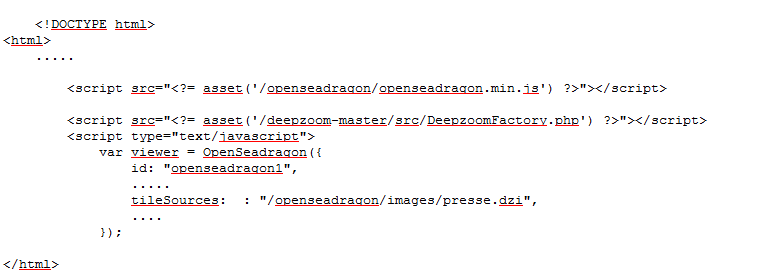
\includegraphics[width=\textwidth]{figure/osd.png}
            \caption{Appel à OpenSeadragon}
            \label{seadragon}
    \end{figure}
	
		  \begin{figure}[H]
        \centering
        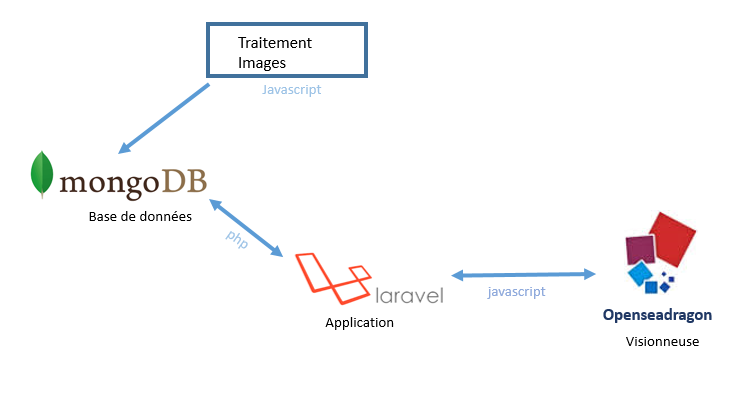
\includegraphics[width=\textwidth]{figure/osdarchi.png}
            \caption{Communication OpenSeadragon/Laravel/MongoDB}
            \label{seadragonarchi}
    \end{figure}




